% CHU SO HUU: Ngọc Dư | KHONG THEO PREAMBLE, KHONG BEGIN DOCUMENT TRONG THAN PHAN NAY.
\section{Kết quả huấn luyện và đánh giá hồi quy Logistic}
\label{sec:t4:result}

Phần này trình bày kết quả thực nghiệm của hồi quy Logistic trên hai tập dữ liệu \texttt{KDDTrain+} ($n=125.973$) và \texttt{KDDTest+} ($n=22.544$). Nội dung gồm: quá trình lựa chọn siêu tham số điều chuẩn qua kiểm định chéo trên tập huấn luyện; phân tích và diễn giải hệ số của mô hình diễn giải; đánh giá khả năng phân loại tổng thể; và phân tích chi tiết các trường hợp phân loại sai theo nhóm tấn công, mức độ quen thuộc của tấn công và độ khó ghi nhận trong dữ liệu.

\subsection{Lựa chọn siêu tham số và kết quả kiểm định chéo}
Mô hình dự đoán (Mô hình B) tiếp nhận toàn bộ 121 đặc trưng đầu vào sau khi biến đổi. Nhằm kiểm soát hiện tượng đa cộng tuyến từ 9 cặp biến tỷ lệ lỗi có $|r|>0{,}95$ và tránh suy giảm nghiệm do các biến giả thưa thớt, kiểm định chéo phân tầng 5 phần (\textit{Stratified 5-Fold Cross-Validation}) được thực hiện độc lập trên tập Train để chọn hệ số điều chuẩn $C\in\{0{,}001;\,0{,}01;\,0{,}1;\,1;\,10;\,100\}$. Bảng~\ref{tab:t4:cv} tổng hợp các độ đo trung bình và sai số chuẩn qua 5 phần kiểm định.

\begin{table}[H]
\centering
\caption{Kết quả kiểm định chéo 5 phần trên tập KDDTrain+ của Mô hình B}
\label{tab:t4:cv}
\small
\setlength{\tabcolsep}{4pt}
\resizebox{\textwidth}{!}{%
\begin{tabular}{rrrrrrr}
\toprule
$C$ & $F_1$ trung bình & $SE(F_1)$ & Accuracy & $SE(\text{Acc})$ & ROC-AUC & $SE(\text{AUC})$ \\
\midrule
0,001 & 0,9663 & 0,0005 & 0,9688 & 0,0004 & 0,9957 & 0,0002 \\
0,010 & 0,9791 & 0,0006 & 0,9806 & 0,0006 & 0,9971 & 0,0002 \\
0,100 & 0,9819 & 0,0004 & 0,9832 & 0,0004 & 0,9976 & 0,0001 \\
1,000 & 0,9835 & 0,0005 & 0,9847 & 0,0004 & 0,9978 & 0,0001 \\
10,000 & \textbf{0,9844} & 0,0005 & 0,9855 & 0,0005 & 0,9979 & 0,0001 \\
100,000 & 0,9844 & 0,0005 & 0,9855 & 0,0004 & 0,9979 & 0,0001 \\
\bottomrule
\end{tabular}%
}
\par\smallskip\footnotesize $SE = \text{Độ lệch chuẩn} / \sqrt{5}$. Giá trị $C=10$ được lựa chọn theo quy tắc một sai số chuẩn (1-SE rule), bảo đảm mức độ điều chuẩn mạnh hơn trong khi $F_1$ sai khác không đáng kể so với $C=100$.
\end{table}

Khi $C$ tăng từ 0,001 lên 10, chỉ số $F_1$ trung bình tăng từ 0,9663 lên 0,9844. Khi tăng tiếp lên $C=100$, đồ thị $F_1$ đạt trạng thái bình nguyên ($F_1$ đạt 0,98442, chỉ tăng $5\times 10^{-5}$). Áp dụng quy tắc một sai số chuẩn (\textit{one-standard-error rule}) \cite{task4_hastie2009}, mức $C=10$ được cố định cho mô hình cuối cùng nhằm ưu tiên nghiệm có tính điều chuẩn cao hơn, tránh khuếch đại các trọng số ở biến hiếm.

\subsection{Ước lượng và diễn giải hệ số mô hình hồi quy Logistic}
Để bảo đảm tính khả giải và tránh sai lệch ước lượng do đa cộng tuyến nặng, Mô hình A sử dụng 9 biến số liên tục (được chuẩn hóa $z$) và 2 biến giả của \texttt{protocol\_type} (với \texttt{tcp} làm mức tham chiếu). Bảng~\ref{tab:t4:coefA} trình bày chi tiết các hệ số hồi quy $\hat\beta_j$, sai số chuẩn $\widehat{SE}$, thống kê Wald $z$, giá trị $p$, tỷ số odds ($OR$) và khoảng tin cậy 95\% tương ứng.

\begin{table}[H]
\centering
\caption{Ước lượng tham số và tỷ số odds của Mô hình A (statsmodels Logit)}
\label{tab:t4:coefA}
\small
\setlength{\tabcolsep}{3pt}
\resizebox{\textwidth}{!}{%
\begin{tabular}{lrrrrrrr}
\toprule
Biến đặc trưng & $\hat\beta_j$ & $\widehat{SE}$ & $z$ (Wald) & $p$-value & $OR_j$ & CI 95\% $OR$ & VIF \\
\midrule
Hệ số chặn (\texttt{const}) & $-0{,}0336$ & 0,0249 & $-1{,}35$ & 0,1781 & 0,967 & $[0{,}921;\ 1{,}015]$ & --- \\
\texttt{src\_bytes} & $-0{,}1961$ & 0,0220 & $-8{,}91$ & $<0{,}001$ & 0,822 & $[0{,}787;\ 0{,}858]$ & 5,09 \\
\texttt{dst\_bytes} & $-0{,}5079$ & 0,0206 & $-24{,}62$ & $<0{,}001$ & 0,602 & $[0{,}578;\ 0{,}627]$ & 3,88 \\
\texttt{count} & $1{,}1815$ & 0,0229 & $51{,}60$ & $<0{,}001$ & 3,259 & $[3{,}116;\ 3{,}409]$ & 3,11 \\
\texttt{dst\_host\_srv\_count} & $-1{,}0452$ & 0,0175 & $-59{,}66$ & $<0{,}001$ & 0,352 & $[0{,}340;\ 0{,}364]$ & 2,92 \\
\texttt{serror\_rate} & $1{,}8013$ & 0,0320 & $56{,}37$ & $<0{,}001$ & 6,057 & $[5{,}690;\ 6{,}449]$ & 9,38 \\
\texttt{rerror\_rate} & $0{,}6178$ & 0,0191 & $32{,}28$ & $<0{,}001$ & 1,855 & $[1{,}787;\ 1{,}926]$ & 4,49 \\
\texttt{same\_srv\_rate} & $-0{,}5348$ & 0,0338 & $-15{,}82$ & $<0{,}001$ & 0,586 & $[0{,}548;\ 0{,}626]$ & 8,31 \\
\texttt{diff\_srv\_rate} & $-0{,}3988$ & 0,0139 & $-28{,}65$ & $<0{,}001$ & 0,671 & $[0{,}653;\ 0{,}690]$ & 1,48 \\
\texttt{dst\_host\_same\_src\_port\_rate} & $0{,}6454$ & 0,0132 & $48{,}84$ & $<0{,}001$ & 1,907 & $[1{,}858;\ 1{,}957]$ & 2,11 \\
\texttt{protocol\_type\_icmp} & $2{,}7221$ & 0,0522 & $52{,}15$ & $<0{,}001$ & 15,213 & $[13{,}733;\ 16{,}851]$ & 2,27 \\
\texttt{protocol\_type\_udp} & $-0{,}6463$ & 0,0466 & $-13{,}88$ & $<0{,}001$ & 0,524 & $[0{,}478;\ 0{,}574]$ & 1,95 \\
\bottomrule
\end{tabular}%
}
\par\smallskip\footnotesize Thống kê tỷ số hợp lý $G = 134.954{,}4$ ($df=11$, $p<0{,}001$). Pseudo-$R^2$ McFadden $= 0{,}7755$; $\text{AIC}=39.102{,}1$; $\text{BIC}=39.219{,}1$. Mức tham chiếu của giao thức là \texttt{tcp}. Toàn bộ $\text{VIF} < 10$.
\end{table}

Kiểm định tỷ số hợp lý cho thấy mô hình có ý nghĩa thống kê vượt trội so với mô hình rỗng ($G=134.954{,}4$, $p<0{,}001$). Hệ số xác định giả McFadden đạt $R^2_{\text{McF}}=0{,}7755$, phản ánh mức độ giải thích biến thiên rất cao. Kiểm tra đa cộng tuyến cho thấy tất cả các biến đều có $\text{VIF}<10$ (cao nhất là \texttt{serror\_rate} với $\text{VIF}=9{,}38$ và \texttt{same\_srv\_rate} với $\text{VIF}=8{,}31$), bảo đảm độ tin cậy của sai số chuẩn và ước lượng Wald.

Hình~\ref{fig:t4:or} trực quan hóa các tỷ số odds và khoảng tin cậy 95\% trên thang đo logarit. Từ bảng kết quả và biểu đồ, các phát hiện thống kê mang ý nghĩa an ninh mạng nổi bật gồm:
\begin{figure}[H]
\centering
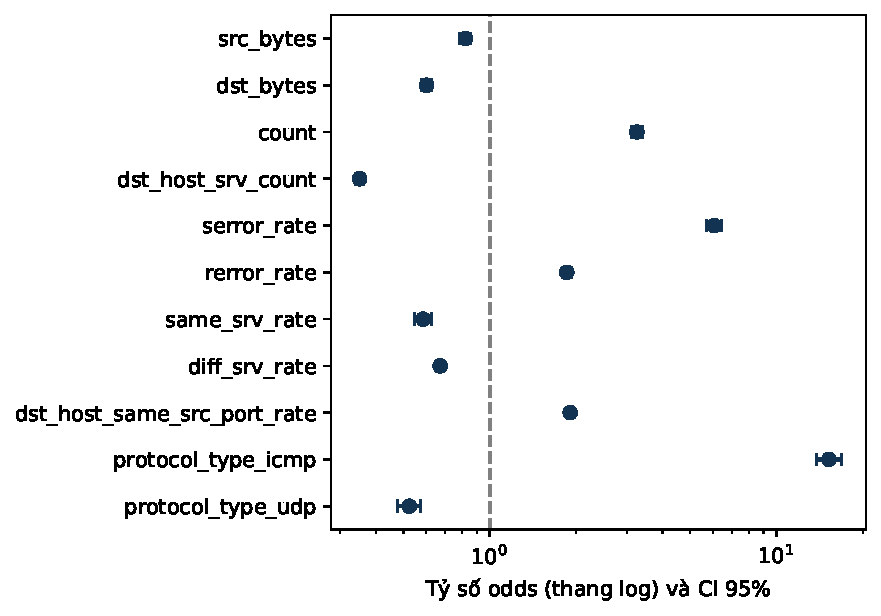
\includegraphics[width=0.72\textwidth]{figures/task4_or_modelA.pdf}
\caption{Biểu đồ khoảng tin cậy 95\% của tỷ số odds ($OR$) trong Mô hình A (thang log)}
\label{fig:t4:or}
\end{figure}

\begin{enumerate}[leftmargin=1.2cm,itemsep=3pt]
\item \textbf{Dấu hiệu bùng nổ lỗi kết nối:} Biến \texttt{serror\_rate} có liên hệ thuận mạnh nhất trong số các biến liên tục ($\hat\beta=1{,}8013$, $OR=6{,}057$, CI 95\%: $[5{,}690;\ 6{,}449]$). Giữ nguyên các biến khác, khi tỷ lệ lỗi SYN trong 2 giây tăng thêm một độ lệch chuẩn, odds của kết nối là tấn công tăng gấp 6,06 lần. Tương tự, tỷ lệ từ chối \texttt{rerror\_rate} có $OR=1{,}855$ ($p<0{,}001$). Đây là dấu hiệu kinh điển của các cuộc tấn công DoS kiểu SYN flood (như \texttt{neptune}) và quét cổng dò tìm dịch vụ đóng.
\item \textbf{Mật độ kết nối lặp lại:} Biến \texttt{count} (số kết nối tới cùng máy đích trong 2 giây) có $\hat\beta=1{,}1815$ ($OR=3{,}259$, CI 95\%: $[3{,}116;\ 3{,}409]$), cho thấy lưu lượng dồn dập trong thời gian ngắn là chỉ báo nguy cơ xâm nhập rất cao. Ngược lại, biến \texttt{dst\_host\_srv\_count} (số kết nối lịch sử cùng máy đích và dịch vụ) có $OR=0{,}352$ ($p<0<001$). Các kết nối hướng tới dịch vụ đã có lịch sử tương tác bền vững thường là lưu lượng hợp lệ (như lướt web kéo dài).
\item \textbf{Khối lượng truyền tải dữ liệu:} Cả \texttt{src\_bytes} ($OR=0{,}822$) và \texttt{dst\_bytes} ($OR=0{,}602$) đều có hệ số âm có ý nghĩa ($p<0{,}001$). Điều này giải thích bởi đặc điểm dữ liệu: phần lớn tấn công DoS và Probe diễn ra rất nhanh, ngắt kết nối giữa chừng hoặc chỉ gửi gói tin mào đầu rỗng, do đó lượng byte truyền tải thực tế thường nhỏ hơn nhiều so với các phiên tải tệp hay truyền nội dung bình thường.
\item \textbf{Loại giao thức truyền thông:} So với giao thức chuẩn \texttt{tcp}, kết nối \texttt{icmp} có odds bị tấn công cao gấp 15,21 lần ($OR=15{,}213$, CI 95\%: $[13{,}733;\ 16{,}851]$), do phần lớn lưu lượng ICMP trong dữ liệu NSL-KDD thuộc về các đợt càn quét mạng (\texttt{ipsweep}) hoặc tấn công từ chối dịch vụ (\texttt{smurf}). Ngược lại, giao thức \texttt{udp} có $OR=0{,}524$, gắn liền nhiều hơn với lưu lượng bình thường (như DNS \texttt{domain\_u}).
\end{enumerate}

\subsection{Đánh giá hiệu năng phân loại trên tập Train và Test}
Mô hình dự đoán B (121 biến đầu vào, $C=10$) và Mô hình diễn giải A (11 biến) được đánh giá trên cả tập huấn luyện và tập kiểm tra độc lập tại ngưỡng quyết định cố định $\hat\pi \geq 0{,}5$. Bảng~\ref{tab:t4:metrics} tổng hợp đầy đủ các chỉ số đánh giá kèm khoảng tin cậy Wilson 95\%.

\begin{table}[H]
\centering
\caption{Độ đo đánh giá hiệu năng phân loại của hai mô hình trên Train và Test}
\label{tab:t4:metrics}
\small
\setlength{\tabcolsep}{3pt}
\resizebox{\textwidth}{!}{%
\begin{tabular}{llrrrrrrr}
\toprule
Mô hình & Tập dữ liệu & $n$ & Accuracy & Precision & Recall & Specificity & $F_1$-score & ROC-AUC \\
\midrule
\textbf{Mô hình B} & Train & 125.973 & 0,9857 & 0,9861 & 0,9831 & 0,9880 & 0,9846 & 0,9980 \\
(Toàn phần) & & & $[0{,}9850; 0{,}9863]$ & $[0{,}9851; 0{,}9870]$ & $[0{,}9820; 0{,}9841]$ & $[0{,}9871; 0{,}9888]$ & --- & --- \\
& Test & 22.544 & \textbf{0,7478} & \textbf{0,9141} & \textbf{0,6147} & \textbf{0,9237} & \textbf{0,7351} & \textbf{0,7878} \\
& & & $[0{,}7421; 0{,}7535]$ & $[0{,}9080; 0{,}9199]$ & $[0{,}6063; 0{,}6231]$ & $[0{,}9182; 0{,}9288]$ & --- & --- \\
\midrule
\textbf{Mô hình A} & Train & 125.973 & 0,9513 & 0,9564 & 0,9380 & 0,9628 & 0,9471 & 0,9775 \\
(Tập gọn) & & & $[0{,}9501; 0{,}9524]$ & $[0{,}9547; 0{,}9581]$ & $[0{,}9360; 0{,}9399]$ & $[0{,}9613; 0{,}9642]$ & --- & --- \\
& Test & 22.544 & 0,7454 & 0,9501 & 0,5834 & 0,9595 & 0,7229 & 0,8249 \\
& & & $[0{,}7397; 0{,}7511]$ & $[0{,}9451; 0{,}9547]$ & $[0{,}5749; 0{,}5919]$ & $[0{,}9554; 0{,}9633]$ & --- & --- \\
\bottomrule
\end{tabular}%
}
\par\smallskip\footnotesize Các khoảng trong ngoặc vuông là khoảng tin cậy Wilson 95\%. Ngưỡng phân loại là 0,5. Lớp dương tính là Attack ($Y=1$).
\end{table}

Trên tập huấn luyện KDDTrain+, Mô hình B đạt hiệu năng gần như hoàn hảo với độ chính xác 98,57\%, $F_1=0{,}9846$ và ROC-AUC đạt 0,9980. Tuy nhiên, khi chuyển sang đánh giá trên KDDTest+, hiệu năng sụt giảm rõ rệt: Accuracy giảm xuống 74,78\% (CI 95\%: $[74,21\%;\ 75,35\%]$) và Recall giảm sâu xuống mức 61,47\% (CI 95\%: $[60,63\%;\ 62,31\%]$). Trong khi đó, Specificity (khả năng nhận diện chính xác lưu lượng Normal) vẫn duy trì ở mức cao đạt 92,37\% và Precision đạt 91,41\%.

\begin{figure}[H]
\centering
\begin{subfigure}[b]{0.48\textwidth}
\centering
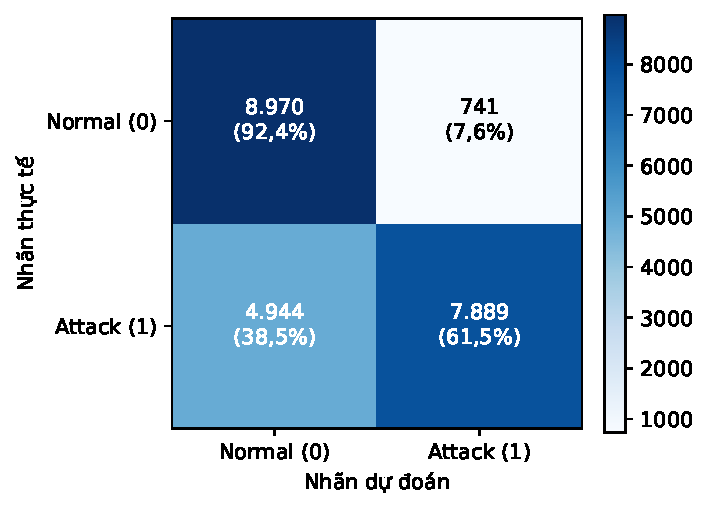
\includegraphics[width=\textwidth]{figures/task4_confusion_test.pdf}
\caption{Ma trận nhầm lẫn của Mô hình B trên KDDTest+}
\label{fig:t4:confusion}
\end{subfigure}
\hfill
\begin{subfigure}[b]{0.48\textwidth}
\centering
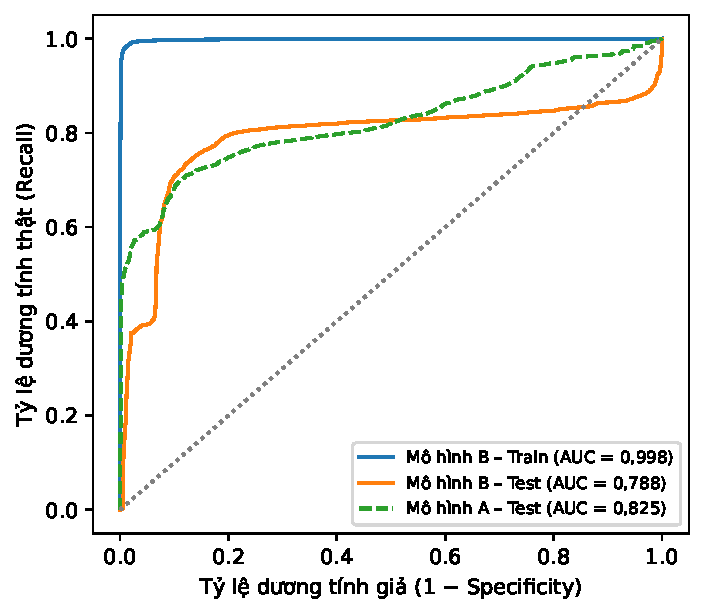
\includegraphics[width=\textwidth]{figures/task4_roc.pdf}
\caption{Đường cong ROC của các mô hình}
\label{fig:t4:roc}
\end{subfigure}
\caption{Hiệu năng phân loại trên tập kiểm tra độc lập KDDTest+}
\end{figure}

Hình~\ref{fig:t4:confusion} thể hiện ma trận nhầm lẫn của Mô hình B trên 22.544 dòng Test:
\begin{itemize}[leftmargin=1.2cm,itemsep=2pt]
\item $TP = 7.889$ kết nối tấn công được phát hiện chính xác (61,5\% số cuộc tấn công).
\item $TN = 8.970$ kết nối bình thường được xác định đúng (92,4\% số kết nối bình thường).
\item $FP = 741$ kết nối bình thường bị gán nhầm là tấn công (tỷ lệ dương tính giả $FPR=7,63\%$).
\item $FN = 4.944$ kết nối tấn công bị bỏ sót hoàn toàn (chiếm 38,5\% tổng số tấn công trong tập Test).
\end{itemize}

Hình~\ref{fig:t4:roc} minh họa đường cong ROC. Trên tập Train, đường ROC áp sát góc trên bên trái ($\text{AUC}=0{,}998$). Trên tập Test, đường ROC của Mô hình B đạt $\text{AUC}=0{,}7878$, phản ánh sự sụt giảm năng lực xếp hạng xác suất khi đối mặt với phân phối lưu lượng mới. Điều đáng chú ý là Mô hình A (tập biến gọn) tuy có Recall thấp hơn ở ngưỡng 0,5 (58,34\%) nhưng đường cong ROC tổng thể trên Test lại đạt $\text{AUC}=0{,}8249$, cao hơn Mô hình B. Hiện tượng này chứng minh mô hình đơn giản ít bị quá khớp (\textit{overfitting}) với các biến giả đặc thù của tập Train hơn mô hình 121 biến.

\subsection{Phân tích các trường hợp phân loại sai (Error Analysis)}
Để giải đáp lý do tỷ lệ Recall trên tập Test giảm xuống 61,47\% và nguồn gốc của 4.944 trường hợp âm tính giả ($FN$), nghiên cứu phân tích chi tiết lỗi theo ba chiều: danh mục tấn công, tính mới của loại tấn công và mức độ khó phân loại.

\subsubsection{Phân tích độ nhạy theo từng nhóm tấn công}
Bảng~\ref{tab:t4:cat} và Hình~\ref{fig:t4:recall_cat} đối chiếu tỷ lệ phân loại đúng giữa tập Train và Test trên 5 nhóm lưu lượng. 

\begin{table}[H]
\centering
\caption{Tỷ lệ phân loại đúng theo từng nhóm lưu lượng trên Train và Test}
\label{tab:t4:cat}
\small
\setlength{\tabcolsep}{4pt}
\resizebox{\textwidth}{!}{%
\begin{tabular}{llrrrrr}
\toprule
Tập & Nhóm & Quy mô ($n$) & Nhận đúng & Bỏ sót & Tỷ lệ (\%) & Khoảng tin cậy 95\% \\
\midrule
Train & Normal & 67.343 & 66.532 & 811 & 98,80 (Specificity) & $[98{,}71;\ 98{,}88]$ \\
& DoS & 45.927 & 45.848 & 79 & 99,83 (Recall) & $[99{,}79;\ 99{,}86]$ \\
& Probe & 11.656 & 11.369 & 287 & 97,54 (Recall) & $[97{,}24;\ 97{,}80]$ \\
& R2L & 995 & 391 & 604 & 39,30 (Recall) & $[36{,}31;\ 42{,}37]$ \\
& U2R & 52 & 32 & 20 & 61,54 (Recall) & $[47{,}96;\ 73{,}53]$ \\
\midrule
Test & Normal & 9.711 & 8.970 & 741 & 92,37 (Specificity) & $[91{,}82;\ 92{,}88]$ \\
& DoS & 7.460 & 5.930 & 1.530 & 79,49 (Recall) & $[78{,}56;\ 80{,}39]$ \\
& Probe & 2.421 & 1.854 & 567 & 76,58 (Recall) & $[74{,}85;\ 78{,}22]$ \\
& R2L & 2.885 & 78 & 2.807 & \textbf{2,70} (Recall) & $[2{,}17;\ 3{,}36]$ \\
& U2R & 67 & 27 & 40 & 40,30 (Recall) & $[29{,}39;\ 52{,}26]$ \\
\bottomrule
\end{tabular}%
}
\par\smallskip\footnotesize Đối với Normal, tỷ lệ đúng là Specificity; đối với 4 nhóm tấn công, tỷ lệ đúng là Recall. Khoảng tin cậy Wilson 95\%.
\end{table}

\begin{figure}[H]
\centering
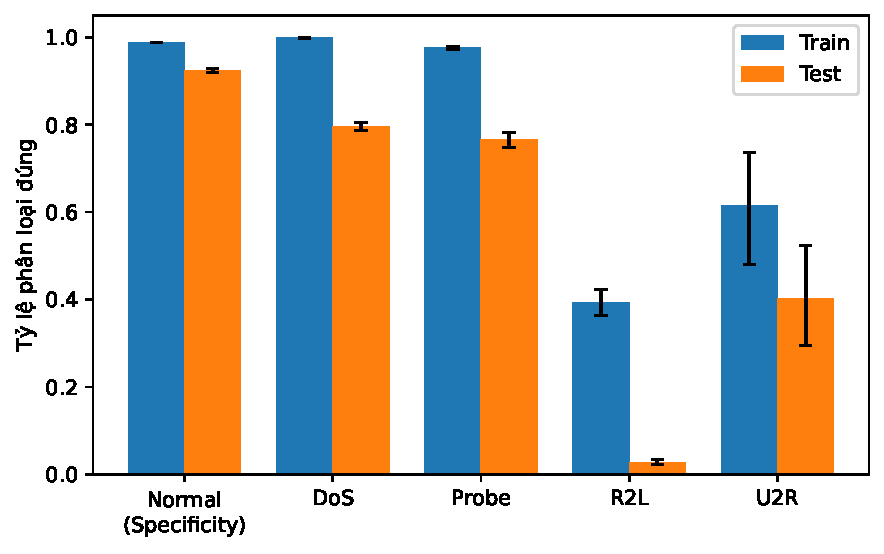
\includegraphics[width=0.75\textwidth]{figures/task4_recall_by_category.pdf}
\caption{So sánh tỷ lệ phân loại đúng giữa Train và Test theo từng nhóm (thanh sai số Wilson 95\%)}
\label{fig:t4:recall_cat}
\end{figure}

Sự sụt giảm hiệu năng tập trung nghiêm trọng nhất ở hai nhóm:
\begin{itemize}[leftmargin=1.2cm,itemsep=3pt]
\item \textbf{Nhóm R2L (Remote to Local):} Tỷ lệ nhận diện trên Test sụp đổ hoàn toàn, chỉ đạt \textbf{2,70\%} (CI 95\%: $[2{,}17\%;\ 3{,}36\%]$), bỏ sót tới 2.807 trên tổng số 2.885 kết nối. Đáng chú ý, các cuộc tấn công R2L chiếm tới 56,8\% trong tổng số 4.944 ca âm tính giả của mô hình. Tấn công R2L (như đoán mật khẩu \texttt{guess\_passwd}) sử dụng các gói tin tương tác bình thường ở tầng ứng dụng, hoàn toàn không gây đột biến số lượng gói tin hay tạo lỗi cờ mạng, khiến bộ phân loại tuyến tính dựa trên các đặc trưng thống kê kết nối không thể phân biệt được.
\item \textbf{Nhóm DoS:} Dù giữ được độ nhạy 79,49\%, nhóm DoS vẫn ghi nhận 1.530 ca bỏ sót, chiếm 31,0\% tổng số FN. Khác với cuộc tấn công \texttt{neptune} quen thuộc trong Train (được phát hiện 99,25\%), các ca bỏ sót thuộc về các dạng DoS ứng dụng mới như \texttt{processtable} và \texttt{apache2}.
\end{itemize}

\subsubsection{Tác động của các biến thể tấn công mới trong KDDTest+}
Một đặc thù cốt lõi của bộ dữ liệu NSL-KDD là tập Test có 17 nhãn tấn công chưa từng xuất hiện trong tập Train, chiếm 3.750 dòng dữ liệu (như đã ghi nhận ở Chương~2). Bảng~\ref{tab:t4:seen} làm rõ độ nhạy phân tách giữa các dạng tấn công cũ và mới.

\begin{table}[H]
\centering
\caption{Khả năng phát hiện các dạng tấn công đã học và tấn công mới trên KDDTest+}
\label{tab:t4:seen}
\small
\setlength{\tabcolsep}{4pt}
\resizebox{\textwidth}{!}{%
\begin{tabular}{lrrrrr}
\toprule
Phân nhóm tấn công & Số lượng ($n$) & Nhận diện ($TP$) & Bỏ sót ($FN$) & Recall (\%) & Khoảng tin cậy 95\% \\
\midrule
Đã có trong Train & 9.083 & 6.865 & 2.218 & \textbf{75,58\%} & $[74{,}69\%;\ 76{,}45\%]$ \\
Chỉ có trong Test (Mới) & 3.750 & 1.024 & 2.726 & \textbf{27,31\%} & $[25{,}90\%;\ 28{,}76\%]$ \\
\bottomrule
\end{tabular}%
}
\par\smallskip\footnotesize Khoảng tin cậy Wilson 95\% cho tỷ lệ Recall.
\end{table}

Kết quả cho thấy khả năng phát hiện các dạng tấn công mới chỉ đạt \textbf{27,31\%}, thấp hơn gần 3 lần so với các dạng tấn công đã có trong tập huấn luyện (75,58\%). Đặc biệt, trong 4.944 ca âm tính giả toàn tập Test, có tới \textbf{2.726 ca (chiếm 55,1\%)} xuất phát từ 17 dạng tấn công mới này. Bảng~\ref{tab:t4:top_missed} liệt kê các loại tấn công bị bỏ sót nhiều nhất.

\begin{table}[H]
\centering
\caption{Danh sách các dạng tấn công bị bỏ sót nhiều nhất trên KDDTest+}
\label{tab:t4:top_missed}
\small
\setlength{\tabcolsep}{4pt}
\resizebox{\textwidth}{!}{%
\begin{tabular}{llrrrrl}
\toprule
Tên tấn công & Nhóm & Tổng số ($n$) & Nhận diện & Bỏ sót ($FN$) & Recall (\%) & Xuất hiện ở Train? \\
\midrule
\texttt{guess\_passwd} & R2L & 1.231 & 0 & 1.231 & 0,00\% & Có (53 dòng) \\
\texttt{warezmaster} & R2L & 944 & 69 & 875 & 7,31\% & Có (20 dòng) \\
\texttt{processtable} & DoS & 685 & 0 & 685 & 0,00\% & Không (Tấn công mới) \\
\texttt{mscan} & Probe & 996 & 455 & 541 & 45,68\% & Không (Tấn công mới) \\
\texttt{apache2} & DoS & 737 & 246 & 491 & 33,38\% & Không (Tấn công mới) \\
\texttt{snmpguess} & R2L & 331 & 3 & 328 & 0,91\% & Không (Tấn công mới) \\
\texttt{mailbomb} & DoS & 293 & 0 & 293 & 0,00\% & Không (Tấn công mới) \\
\texttt{snmpgetattack} & R2L & 178 & 1 & 177 & 0,56\% & Không (Tấn công mới) \\
\texttt{httptunnel} & R2L & 133 & 2 & 131 & 1,50\% & Không (Tấn công mới) \\
\bottomrule
\end{tabular}%
}
\end{table}

Đáng chú ý, hai cuộc tấn công R2L có mặt trong Train là \texttt{guess\_passwd} (1.231 quan sát) và \texttt{warezmaster} (944 quan sát) bị bỏ sót gần như 100\%. Lý do là trong tập Train, hai nhãn này chỉ chiếm lần lượt 53 dòng và 20 dòng (tỷ lệ dưới 0,05\%), mô hình hồi quy logistic tuyến tính với hàm mất mát chuẩn không được cung cấp đủ trọng số để học ranh giới cho các lớp thiểu số cực đoan này.

\subsubsection{Mối quan hệ giữa độ khó (difficulty) và độ chính xác}
Chỉ số \texttt{difficulty} (0--21) đo lường số lượng mô hình máy học nguyên bản trong nghiên cứu của Tavallaee và cộng sự \cite{task1_tavallaee2009} đã dự đoán đúng kết nối. Dù không được sử dụng làm biến dự đoán, biến này là công cụ kiểm chuẩn tuyệt vời sau mô hình. Bảng~\ref{tab:t4:diff} thống kê độ chính xác của Mô hình B theo các khoảng độ khó.

\begin{table}[H]
\centering
\caption{Độ chính xác phân loại của Mô hình B theo mức độ khó trên KDDTest+}
\label{tab:t4:diff}
\small
\setlength{\tabcolsep}{4pt}
\resizebox{\textwidth}{!}{%
\begin{tabular}{lrrrrr}
\toprule
Khoảng độ khó & Số quan sát ($n$) & Tấn công thực & Dự đoán đúng & Accuracy (\%) & Khoảng tin cậy 95\% \\
\midrule
$0 - 10$ (Rất khó) & 1.423 & 1.171 & 123 & \textbf{8,64\%} & $[7{,}29\%;\ 10{,}22\%]$ \\
$11 - 15$ (Khó) & 3.378 & 3.215 & 955 & \textbf{28,27\%} & $[26{,}78\%;\ 29{,}81\%]$ \\
$16 - 20$ (Trung bình) & 7.049 & 5.312 & 5.101 & \textbf{72,36\%} & $[71{,}31\%;\ 73{,}40\%]$ \\
$21$ (Rất dễ) & 10.694 & 3.135 & 10.680 & \textbf{99,87\%} & $[99{,}78\%;\ 99{,}92\%]$ \\
\bottomrule
\end{tabular}%
}
\par\smallskip\footnotesize Khoảng tin cậy Wilson 95\% cho Accuracy.
\end{table}

Độ chính xác phân loại tăng đơn điệu tuyệt đối theo thang độ khó: từ 8,64\% ở nhóm khó nhất ($0-10$) lên đến 99,87\% ở nhóm kết nối dễ phân loại nhất (mức 21). Điều này xác nhận rằng các ca lỗi của hồi quy Logistic hoàn toàn đồng nhất với các điểm mù cố hữu của các mô hình phân loại mạng truyền thống trên NSL-KDD.

\subsubsection{Mức độ tự tin của mô hình và phân tích báo động giả (FP)}
Hình~\ref{fig:t4:prob_hist} thể hiện biểu đồ phân bố xác suất dự đoán $\hat\pi$ của Mô hình B trên KDDTest+ theo nhãn thực tế.

\begin{figure}[H]
\centering
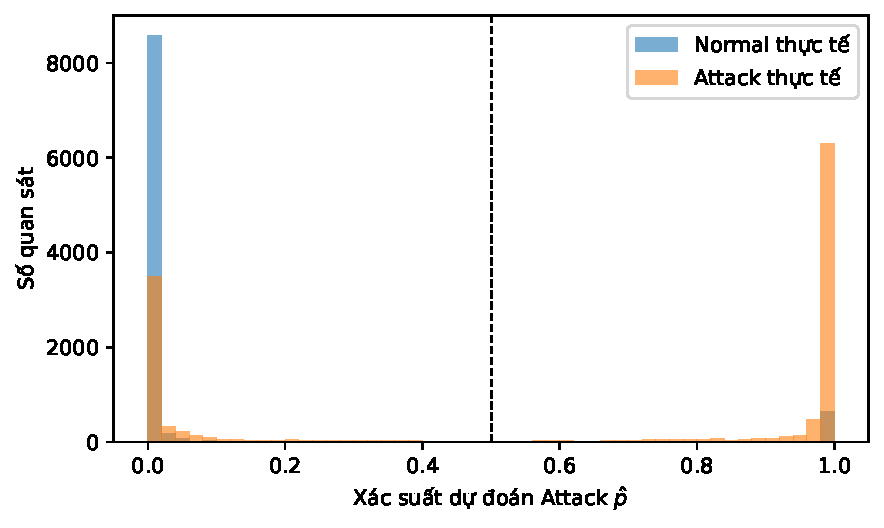
\includegraphics[width=0.72\textwidth]{figures/task4_prob_hist_test.pdf}
\caption{Phân bố xác suất dự đoán Attack ($\hat\pi$) trên KDDTest+ phân tách theo nhãn thực}
\label{fig:t4:prob_hist}
\end{figure}

Phân bố cho thấy hai đỉnh nhọn cực đoan ở sát 0 và 1. Đặc biệt, trung vị xác suất dự đoán của 4.944 ca âm tính giả ($FN$) chỉ là \textbf{0,00064}, và có tới \textbf{87,0\% số ca $FN$ có xác suất dự đoán $\hat\pi < 0{,}1$}. Điều này chỉ ra rằng mô hình không hề ``lưỡng lự'' quanh ngưỡng cắt 0,5, mà hoàn toàn tự tin kết luận các cuộc tấn công này là Normal. Vì vậy, việc tinh chỉnh hay hạ ngưỡng quyết định không thể giải quyết được các ca bỏ sót này mà chỉ làm bùng nổ tỷ lệ báo động giả.

Về phía 741 trường hợp dương tính giả ($FP$ -- Normal bị cảnh báo nhầm):
\begin{itemize}[leftmargin=1.2cm,itemsep=2pt]
\item \textbf{Theo dịch vụ mạng:} Có tới 646 ca (chiếm 87,2\% tổng số FP) xảy ra tại cổng dịch vụ \texttt{service = private}. Trên tập Test, trong 852 kết nối bình thường truy cập dịch vụ private, có tới 646 kết nối bị gán nhầm là tấn công (tỷ lệ báo động giả trên cổng này lên đến 75,82\%). Điều này do trong tập huấn luyện Train, dịch vụ private có tới 20.871 kết nối tấn công và chỉ 982 kết nối bình thường, khiến mô hình học được trọng số dương rất lớn cho biến giả \texttt{service\_private} ($\hat\beta = 3{,}505$, $OR = 33{,}3$).
\item \textbf{Theo cờ kết nối:} 699 ca FP mang cờ kết nối \texttt{SF} (kết nối bình thường) và 35 ca mang cờ \texttt{RSTR} (tỷ lệ lỗi 79,55\% trên tổng số 44 kết nối normal mang cờ này).
\end{itemize}

\subsection{Tiểu kết và ý nghĩa đối với bài toán IDS}
Thực nghiệm Task 4 đã cung cấp các kết luận thống kê quan trọng:
\begin{enumerate}[leftmargin=1.2cm,itemsep=3pt]
\item Hồi quy Logistic tuyến tính thể hiện năng lực xuất sắc trong việc phát hiện các cuộc tấn công quy mô lớn, tần suất cao và phát sinh bất thường ở mức giao vận như DoS (SYN flood \texttt{neptune}) và Probe, với độ nhạy đạt trên 76--79\% và tỷ lệ báo động nhầm tổng thể thấp (Specificity $>92\%$).
\item Hạn chế căn bản của mô hình nằm ở giả định liên kết tuyến tính và sự phụ thuộc vào các đặc trưng mào đầu mạng cấp thấp: mô hình bất lực trước các cuộc tấn công tầng ứng dụng (R2L, Recall chỉ đạt 2,7\%) và suy giảm mạnh năng lực khi gặp các dạng tấn công mới trong thực tế (Recall 27,3\%).
\item Các kết quả định lượng chi tiết này tạo cơ sở vững chắc để nhóm bước vào Chương~5 (Task 5), thảo luận sâu về ưu thế, rào cản và đề xuất các kiến trúc phân loại phi tuyến nâng cao cho hệ thống phát hiện xâm nhập mạng.
\end{enumerate}
\FloatBarrier
